\begin{landscape}
  \singlespacing
  \small\setlength{\tabcolsep}{3pt}
  \def\unsep{\null\hspace{-3pt}\null}
  \begin{longtable}{rllRRlRRl}
    \caption{Definitions and distributions of calibrated parameters}
    \label{tab:par.cal} \\
    \toprule
    & & \multicolumn{4}{c}{Prior} & \multicolumn{3}{c}{Posterior} \\
    \cmidrule(rl){3-6}\cmidrule(rl){7-9}
    Parameter & Definition & Type & Mean & \multicolumn{2}{c}{(95\%~CI)} & Mean & \multicolumn{2}{c}{(95\%~CI)} \\
    \midrule \endfirsthead
    \multicolumn{3}{l}{continued \dots} \\ \midrule \endhead
    \midrule \multicolumn{3}{l}{continued \dots} \\ \endfoot
    \bottomrule \noalign{\vskip\abovecaptionskip} \multicolumn{9}{c}{\begin{minipage}{\linewidth}\footnotesize
    FSW: female sex worker;
    p12m: past 12 months;
    $\beta$: per-act probability of HIV transmission;
    GUD: any genital ulcer disease in p12m;
    ART: antiretroviral therapy;
    VLS: viral load suppression;
    additional relative (aR): relative value beyond one, \eg $R = 1.5 \rightarrow aR = 0.5$;
    prevalence interpolator (iP): \eg $P_0 = 0.2, P_1 = 0.4, iP_x = 0.5 \rightarrow P_x = 0.3$;
    all rates in per-year;
    all durations in years;
    all parameters reflect stratum averages.
    \end{minipage}} \endlastfoot
\texttt{t0_hiv} & year of HIV introduction to Eswatini & Uniform & 1982.5 & (1980.1, & 1984.9) & 1982.6 & (1980.3, & 1985.0) \\
\texttt{PX_w_fsw} & proportion of women who are FSW & Beta & 0.0288 & (0.00703, & 0.065) & 0.0344 & (0.0207, & 0.0526) \\
\texttt{PX_w_h} & proportion of women who have 2+ partners in p12m & Beta & 0.178 & (0.0961, & 0.278) & 0.191 & (0.134, & 0.245) \\
\texttt{PX_m_m} & proportion of men who have 2+ partners in p12m & Beta & 0.133 & (0.1, & 0.17) & 0.137 & (0.103, & 0.164) \\
\texttt{dur_fsw} & duration in sex work overall & Gamma & 4.07 & (2.29, & 6.34) & 3.81 & (2.56, & 5.01) \\
\texttt{dur_sw_h} & duration in higher risk sex work & Gamma & 0.5 & (0.17, & 1.0) & 0.583 & (0.285, & 0.936) \\
\texttt{dur_cli} & duration buying sex among clients & Gamma & 8.63 & (4.0, & 15.0) & 8.79 & (4.89, & 12.7) \\
\texttt{turn_xm_xl} & turnover rate from medium to lowest activity (women and men) & Gamma & 0.216 & (0.05, & 0.5) & 0.231 & (0.11, & 0.443) \\
\texttt{Pturn_fsw_m:l} & proportion of FSW who transition to medium activity & Beta & 0.724 & (0.503, & 0.898) & 0.743 & (0.594, & 0.881) \\
\texttt{Pturn_cli_m:l} & proportion of clients who transition to medium activity & Beta & 0.602 & (0.249, & 0.9) & 0.6 & (0.361, & 0.804) \\
\texttt{growth_2050} & rate of Eswatini population growth in 2050 & Uniform & 0.011 & (0.0072, & 0.0148) & 0.0108 & (0.00737, & 0.0144) \\
\texttt{C12m_msp_xl} & number of main/spousal partners in p12m among lowest activity & Beta & 0.37 & (0.251, & 0.498) & 0.371 & (0.277, & 0.469) \\
\texttt{C12m_cas_xl} & number of casual partners in p12m among lowest activity & Beta & 0.366 & (0.201, & 0.549) & 0.368 & (0.239, & 0.497) \\
\texttt{C12m_cas_wm} & number of casual partners in p12m among medium activity women & Gamma & 1.58 & (1.2, & 2.0) & 1.67 & (1.43, & 1.95) \\
\texttt{RC_cas_cli:wm} & relative casual partners among clients vs medium activity women & Uniform & 0.625 & (0.269, & 0.981) & 0.751 & (0.296, & 1.0) \\
\texttt{C1m_swo_fsw_l} & number of one-off sex work partners in p1m among lower risk FSW & Gamma & 3.5 & (2.27, & 5.0) & 3.28 & (2.45, & 4.34) \\
\texttt{C1m_swr_fsw_l} & number of repeat sex work partners in p1m among lower risk FSW & Gamma & 6.0 & (3.88, & 8.57) & 5.42 & (3.38, & 7.69) \\
\texttt{C1m_swo_fsw_h} & number of one-off sex work partners in p1m among higher risk FSW & Gamma & 14.0 & (9.06, & 20.0) & 13.7 & (9.67, & 17.3) \\
\texttt{C1m_swr_fsw_h} & number of repeat sex work partners in p1m among higher risk FSW & Gamma & 21.0 & (13.6, & 30.0) & 22.7 & (14.8, & 29.2) \\
\texttt{KF_swx_cli} & rate of visiting FSW (sex acts) among clients overall & Gamma & 40.5 & (18.0, & 71.9) & 51.4 & (32.6, & 71.4) \\
\texttt{RKF_swx_cli_h:l} & relative visits (sex acts) among higher vs lower risk clients & Gamma & 2.03 & (1.6, & 2.5) & 2.04 & (1.74, & 2.38) \\
\texttt{F_msp} & rate of sex acts in main/spousal partnerships & Gamma & 77.3 & (26.0, & 156.0) & 86.0 & (56.3, & 123.0) \\
\texttt{RF_cas:msp} & relative rate of sex acts in casual vs main/spousal partnerships & Uniform & 1.25 & (0.538, & 1.96) & 1.6 & (1.0, & 2.0) \\
\texttt{dur_msp} & duration of main/spousal partnerships & Uniform & 16.5 & (14.6, & 18.4) & 16.6 & (15.0, & 18.5) \\
\texttt{dur_cas} & duration of casual partnerships & Gamma & 0.743 & (0.25, & 1.5) & 0.78 & (0.484, & 1.12) \\
\texttt{dur_swr} & duration of repeat sex work partnerships & Gamma & 0.495 & (0.166, & 1.0) & 0.435 & (0.212, & 0.78) \\
\texttt{F_swr} & rate of sex acts in repeat sex work partnerships & Uniform & 24.0 & (12.6, & 35.4) & 20.7 & (12.0, & 32.3) \\
\texttt{PF_ai_mcx} & proportion of anal sex acts in main/spousal and casual partnerships & Gamma & 0.0573 & (0.00603, & 0.165) & 0.114 & (0.0584, & 0.217) \\
\texttt{RPF_ai_swx:mcx} & relative proportion of anal sex acts in sex work vs other partnerships & Uniform & 1.5 & (1.02, & 1.98) & 1.57 & (1.05, & 1.98) \\
\texttt{lpref_msp_xl} & log-odds of main/spousal partnership formation among lowest activity & Uniform & 0 & (-1.9, & 1.9) & -0.217 & (-1.93, & 1.21) \\
\texttt{lpref_mcx_swx} & log-odds of non-sex work partnership formation among FSW and clients & Uniform & 0 & (-1.9, & 1.9) & -0.0689 & (-1.79, & 1.57) \\
\texttt{Rbeta_condom} & relative per-act probability of HIV transmission with a condom & Beta & 0.266 & (0.131, & 0.429) & 0.304 & (0.194, & 0.409) \\
\texttt{RPF_condom_a:v} & relative condom use in anal vs vaginal sex & Beta & 0.768 & (0.504, & 0.949) & 0.733 & (0.553, & 0.903) \\
\texttt{RPF_condom_1996} & elative condom use in all partnerships in 1996 vs 2002 or 2006 & Uniform & 0.5 & (0.025, & 0.975) & 0.53 & (0.054, & 0.998) \\
\texttt{PF_condom_msp_2006} & condom use in main/spousal partnerships in 2006 & Beta & 0.23 & (0.153, & 0.317) & 0.23 & (0.172, & 0.296) \\
\texttt{PF_condom_msp_2016} & condom use in main/spousal partnerships in 2006 & Beta & 0.416 & (0.308, & 0.529) & 0.418 & (0.335, & 0.504) \\
\texttt{PF_condom_cas_2006} & condom use in casual partnerships in 2006 & Beta & 0.598 & (0.501, & 0.692) & 0.594 & (0.53, & 0.671) \\
\texttt{PF_condom_cas_2016} & condom use in casual partnerships in 2016 & Beta & 0.694 & (0.601, & 0.78) & 0.695 & (0.636, & 0.767) \\
\texttt{PF_condom_swo_2002} & condom use in one-off sex work partnerships in 2002 & Beta & 0.432 & (0.148, & 0.744) & 0.486 & (0.254, & 0.762) \\
\texttt{PF_condom_swo_2011} & condom use in one-off sex work partnerships in 2011 & Beta & 0.777 & (0.581, & 0.923) & 0.797 & (0.708, & 0.879) \\
\texttt{PF_condom_swo_2014} & condom use in one-off sex work partnerships in 2014 & Beta & 0.787 & (0.547, & 0.95) & 0.862 & (0.779, & 0.939) \\
\texttt{PF_condom_swr_2002} & condom use in repeat sex work partnerships in 2002 & Beta & 0.337 & (0.118, & 0.603) & 0.294 & (0.126, & 0.485) \\
\texttt{PF_condom_swr_2011} & condom use in repeat sex work partnerships in 2011 & Beta & 0.754 & (0.568, & 0.9) & 0.706 & (0.608, & 0.788) \\
\texttt{PF_condom_swr_2014} & condom use in repeat sex work partnerships in 2014 & Beta & 0.759 & (0.481, & 0.949) & 0.745 & (0.649, & 0.84) \\
\texttt{PF_circum_2050} & prevalence of circumcision by 2050 & Beta & 0.724 & (0.503, & 0.898) & 0.741 & (0.581, & 0.871) \\
\texttt{beta_0} & per-act probability of HIV transmission $\beta$ for CD4 $>$ 350 (REF) & Gamma & 0.00131 & (0.000498, & 0.00251) & 0.00174 & (0.00123, & 0.00247) \\
\texttt{Rbeta_acute} & relative $\beta$ during acute infection & Gamma & 6.01 & (1.11, & 15.0) & 9.33 & (4.98, & 15.8) \\
\texttt{Rbeta_350} & relative $\beta$ for 200 $<$ CD4 $<$ 350 & Gamma & 1.59 & (1.3, & 1.9) & 1.55 & (1.32, & 1.76) \\
\texttt{Rbeta_200} & relative $\beta$ for CD4 $<$ 200 & Gamma & 8.2 & (4.5, & 13.0) & 8.17 & (5.48, & 11.1) \\
\texttt{Rbeta_vi_rec} & relative $\beta$ for receptive vaginal sex & Uniform & 1.5 & (1.02, & 1.98) & 1.66 & (1.21, & 1.99) \\
\texttt{aRbeta_gud_sus} & additional relative $\beta$ for GUD among susceptible partner & Gamma & 2.05 & (0.2, & 6.0) & 2.55 & (0.415, & 5.45) \\
\texttt{aRbeta_gud_inf} & additional relative $\beta$ for GUD among infectious partner & Gamma & 0.99 & (0.2, & 2.4) & 1.04 & (0.272, & 1.99) \\
\texttt{dur_acute} & duration of acute infection & Gamma & 0.172 & (0.0174, & 0.5) & 0.288 & (0.111, & 0.489) \\
\texttt{P_gud_fsw_l} & prevalence of GUD among lower risk FSW & Beta & 0.295 & (0.2, & 0.4) & 0.294 & (0.218, & 0.368) \\
\texttt{RP_gud_fsw_h:l} & relative prevalence of GUD among higher vs lower risk FSW & Gamma & 1.28 & (1.0, & 1.6) & 1.31 & (1.07, & 1.52) \\
\texttt{RP_gud_2030} & relative prevalence of GUD overall in 2030 vs 2010 & Uniform & 0.6 & (0.22, & 0.98) & 0.817 & (0.366, & 1.0) \\
\texttt{iP_gud_h:l} & interpolator for GUD among medium activity vs DHS and FSW & Uniform & 0.5 & (0.025, & 0.975) & 0.518 & (0.0537, & 0.953) \\
\texttt{Rbeta_uvls} & relative $\beta$ on ART but before VLS & Beta & 0.244 & (0.0139, & 0.656) & 0.302 & (0.0656, & 0.614) \\
\texttt{Rdx_global} & relative rate of diagnosis overall & Uniform & 0.75 & (0.512, & 0.988) & 0.645 & (0.536, & 0.775) \\
\texttt{dx_w_2002} & rate of diagnosis among women in 2002 & Beta & 0.094 & (0.0452, & 0.158) & 0.0949 & (0.056, & 0.135) \\
\texttt{dx_w_2006} & rate of diagnosis among women in 2006 & Beta & 0.248 & (0.169, & 0.337) & 0.271 & (0.218, & 0.319) \\
\texttt{Rdx_m:w_2006} & relative rate of diagnosis among men vs women in 2006 & Gamma & 0.377 & (0.207, & 0.597) & 0.471 & (0.333, & 0.66) \\
\texttt{dx_wq_2011} & rate of diagnosis among non-FSW women in 2011 & Gamma & 0.637 & (0.466, & 0.834) & 0.544 & (0.421, & 0.657) \\
\texttt{Rdx_m:wq_2011} & relative rate of diagnosis among men vs non-FSW women in 2011 & Gamma & 0.529 & (0.351, & 0.742) & 0.467 & (0.385, & 0.555) \\
\texttt{aRdx_fsw:wq_2011} & additional relative diagnosis among FSW vs non-FSW women in 2011 & Gamma & 0.521 & (0.206, & 0.98) & 0.542 & (0.301, & 0.854) \\
\texttt{aRdx_wq_16:11} & additional relative diagnosis among non-FSW women in 2016 vs 2011 & Gamma & 0.204 & (0.118, & 0.313) & 0.186 & (0.12, & 0.264) \\
\texttt{aRdx_fsw:wq_2016} & additional relative diagnosis among FSW vs non-FSW women in 2016 & Gamma & 0.619 & (0.291, & 1.07) & 0.589 & (0.416, & 0.848) \\
\texttt{tx_2010} & rate of ART initiation among diagnosed and eligible in 2010 & Gamma & 1.5 & (0.509, & 3.02) & 1.5 & (0.937, & 2.1) \\
\texttt{tx_2012} & rate of ART initiation among diagnosed and eligible in 2012 & Gamma & 8.75 & (6.01, & 12.0) & 7.75 & (5.91, & 9.8) \\
\texttt{Rtx_fsw:wq} & relative rate of ART initiation among FSW vs non-FSW women & Uniform & 0.75 & (0.512, & 0.988) & 0.757 & (0.522, & 0.966) \\
\texttt{ivx} & duration on ART before achieving VLS initially & Gamma & 0.62 & (0.33, & 1.0) & 0.75 & (0.589, & 0.887) \\
\texttt{Runvx_m:wq} & relative rate of viral unsuppression among men vs non-FSW women & Uniform & 1.25 & (1.01, & 1.49) & 1.3 & (1.0, & 1.5) \\
\texttt{Runvx_fsw:wq} & relative rate of viral unsuppression among FSW vs non-FSW women & Uniform & 1.25 & (1.01, & 1.49) & 1.24 & (1.01, & 1.47) \\
\texttt{revx_2010} & rate of viral re-suppression in 2010 & Gamma & 0.729 & (0.5, & 1.0) & 0.609 & (0.492, & 0.788) \\
 %
  \end{longtable}
\end{landscape}
 % MAN: placement
\section{Model Calibration}\label{mod.cal}
We considered uncertainty in 74 model input parameters (Table~\ref{tab:par.cal}).
For each uncertain parameter, we specified a univariate prior distribution
based on the available data and/or assumptions (\sref{mod.par}).
Model calibration aims to reduce this uncertainty
--- \ie estimate the (joint) parameter posterior distribution ---
by comparing model outputs to ``calibration targets''
under different combinations of input parameters.
Table~\ref{tab:par.cal} summarizes the calibrated parameters,
including the mean (95\%~CI) for prior and posterior distributions;
\sref{mod.cal.appr} describes our approach to calibration, and
\sref{mod.cal.targ} details the calibration targets used.
These targets include estimates of HIV incidence, prevalence, and the cascade of care
for the population overall, and stratified by risk group where possible.
Results of model calibration are given in \sref{sr.cal}.
%===================================================================================================
\subsection{Approach}\label{mod.cal.appr}
We used an adapted version of the
Incremental Mixture Importance Sampling (IMIS) procedure \cite{Raftery2010} for model calibration.
% TODO
%---------------------------------------------------------------------------------------------------
\subsubsection{Sampling with Relational Constraints}\label{mod.cal.appr.jsam}
We imposed the following relational constraints on calibrated parameter values during sampling:
\begin{itemize}\singlespacing
  \item[a.] \texttt{K_swo_fsw_h * F_swo + K_swr_fsw_h * F_swr < 2*365}\\
  where: \texttt{K_swx_fsw_h = C1m_swx_fsw_h * dur_swx / (dur_swx + 1/12)}
  \item[b.] Let ``\texttt{c_}'' denote \texttt{PF_condom_}:\\
  \texttt{c_msp_2006 < c_msp_2016}\\
  \texttt{c_cas_2006 < c_cas_2016}\\
  \texttt{c_swo_2002 < c_swo_2011 < c_swo_2014}\\
  \texttt{c_swr_2002 < c_swr_2011 < c_swr_2014}\\
  \texttt{c_msp_2006 < c_cas_2006}\\
  \texttt{c_msp_2016 < c_cas_2016}\\
  \texttt{c_swr_2002 < c_swo_2002}\\
  \texttt{c_swr_2011 < c_swo_2011}\\
  \texttt{c_swr_2014 < c_swo_2014}
  \item[c.] \texttt{1 <= (Rbeta_acute * dur_acute) <= 63}
  \item[d.] \texttt{P_gud_fsw_l > .07}\\
  \texttt{(P_gud_fsw_l * RP_gud_fsw_h:l) < 1}
\end{itemize}
For each set of constraints, parameters were repeatedly sampled until all constraints were satisfied.
As shown in Figure~\ref{fig:jsam.bias},
this approach reduces distortion of sampled \vs prior distributions,
as compared to forward/backward conditional sampling.
Constrained parameters were therefore omitted from initial Latin hypercube sampling.
\begin{figure}[h]
  \centering
  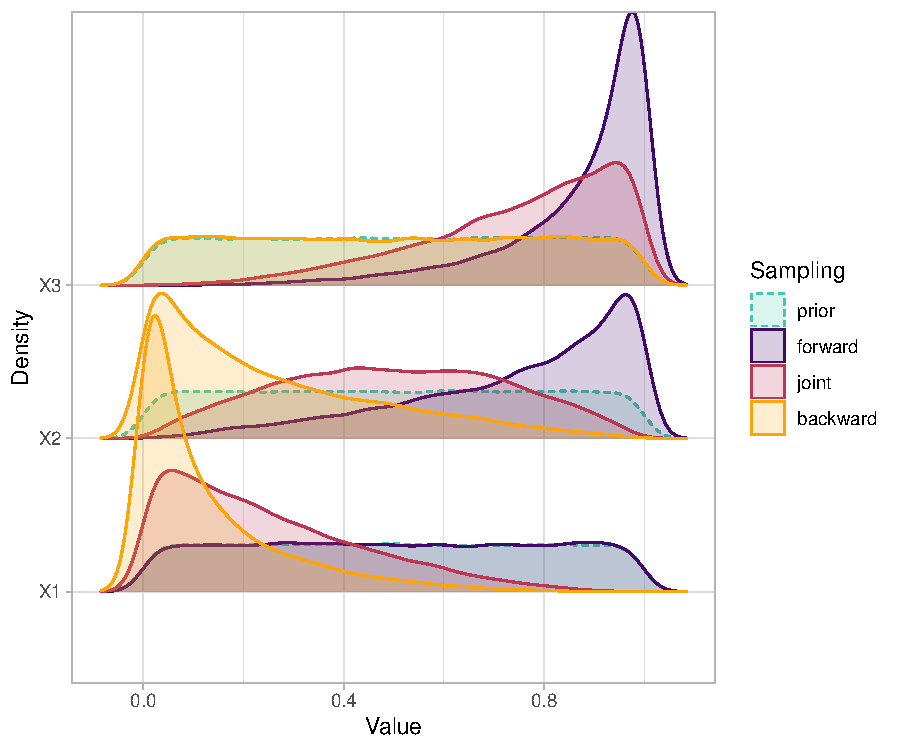
\includegraphics[width=.6\linewidth]{jsam.bias}
  \caption{Illustration of different sampling biases when enforcing $X_1 < X_2 < X_3$}
  \label{fig:jsam.bias}
  \floatfoot{Sampling method:
    \emph{joint:} sample $X_1$, $X_2$, $X_3$ simultaneously; then discard any samples failing $X_1 < X_2 < X_3$;
    \emph{forward:} sample $X_1$; then sample $X_2$ until $X_1 < X_2$; then sample $X_3$ until $X_2 < X_3$;
    \emph{backward:} sample $X_3$; then sample $X_2$ until $X_2 < X_3$; then sample $X_1$ until $X_1 < X_2$.}
\end{figure}

%===================================================================================================
\subsection{Calibration Targets}\label{mod.cal.targ}
The data sources for Eswatini calibration targets
are mainly the same as for Eswatini-specific parameters.
We assumed that population-level surveys in
2006 \cite{SDHS2006}, 2011 \cite{Bicego2013,Justman2016}, and 2016 \cite{SHIMS2}
reached FSW and their clients,
although respondents may not report selling or buying sex in the context of these surveys.
%---------------------------------------------------------------------------------------------------
\subsubsection{HIV Prevalence}\label{mod.cal.targ.prev}
% TODO: (*) clients prevalence ratio Carrasco2020 Table 2
\begin{table}
  \centering
  \caption{Estimates of HIV prevalence in Eswatini}
  \label{tab:targ.prev}
  % TODO: SHIMS3 N = 15+ not 15-49
\begin{tabular}{lcrccccll}
  \toprule
  Population\tn{a} & Year &      N & Raw \%  & Adj \%  &   (95\%~CI)  & Used & Ref & Notes \\
  \midrule
  Overall          & 2006 &  8,187 & 25.9 &  --- & (24.4,~27.3) & \yes & \cite{SDHS2006}   & \tn{b} \\
                   & 2011 & 18,172 & 32.1 & 28.0 & (27.0,~29.0) & \yes & \cite{Bicego2013} & \tn{cd} \\
                   & 2016 &  8,533 & 27.2 &  --- & (25.8,~28.7) & \yes & \cite{SHIMS2}     & \tn{b} \\
                   & 2021 & 12,043 & 23.7 &  --- & (22.6,~24.9) & \yes & \cite{SHIMS3}     & \tn{e} \\[1ex]
  Women Overall    & 2006 &  4,424 & 31.1 &  --- & (29.4,~32.9) & \yes & \cite{SDHS2006}   & \tn{b} \\
                   & 2011 &  9,843 & 38.8 & 34.2 & (33.0,~35.4) & \yes & \cite{Bicego2013} & \tn{cd} \\
                   & 2016 &  4,878 & 34.3 &  --- & (32.6,~36.0) & \yes & \cite{SHIMS2}     & \tn{b} \\
                   & 2021 &  6,985 & 31.6 &  --- & (29.8,~33.4) & \yes & \cite{SHIMS3}     & \tn{e} \\[1ex]
  Men Overall      & 2006 &  3,763 & 19.7 &  --- & (17.9,~21.4) & \yes & \cite{SDHS2006}   & \tn{b} \\
                   & 2011 &  8,329 & 24.1 & 20.7 & (19.6,~21.8) & \yes & \cite{Bicego2013} & \tn{cd} \\
                   & 2016 &  3,655 & 18.8 &  --- & (17.3,~20.4) & \yes & \cite{SHIMS2}     & \tn{b} \\
                   & 2021 &  5,058 & 15.6 &  --- & (14.3,~16.9) & \yes & \cite{SHIMS3}     & \tn{e} \\[1ex]
  LR Overall       & 2006 &  7,589 & 24.9 &  --- &      ---     & \no  & \cite{SDHS2006}   & \\
                   & 2011 & 16,145 & 31.9 &  --- &      ---     & \no  & \cite{Bicego2013} & \\
                   & 2016 &  7,887 & 32.2 &  --- &      ---     & \no  & \cite{SHIMS2}     & \\[1ex]
  Non-LR Overall   & 2006 &    579 & 38.3 &  --- &      ---     & \no  & \cite{SDHS2006}   & \\
                   & 2011 &  1,887 & 33.3 & 29.0 & (25.9,~32.2) & \no  & \cite{Bicego2013} & \tn{cd} \\
                   & 2016 &    914 & 28.7 &  --- & (25.8,~31.7) & \no  & \cite{SHIMS2}     & \tn{g}  \\[1ex]
  LR Women         & 2006 &  4,346 & 30.7 & 26.8 & (22.7,~28.7) & \ast & \cite{SDHS2006}   & \tn{f}  \\
                   & 2011 &  9,843 & 38.2 & 30.8 & (28.9,~32.8) & \ast & \cite{Bicego2013} & \tn{cf} \\
                   & 2016 &  5,203 & 36.5 & 31.5 & (30.0,~33.1) & \ast & \cite{SHIMS2}     & \tn{f}  \\[1ex]
  Non-LR Women     & 2006 &     72 & 53.0 &  --- & (41.5,~64.3) & \ast & \cite{SDHS2006}   & \tn{g}  \\
                   & 2011 &    373 & 54.5 & 48.1 & (41.5,~54.8) & \ast & \cite{Bicego2013} & \tn{cd} \\
                   & 2016 &    263 & 45.3 &  --- & (39.3,~51.3) & \ast & \cite{SHIMS2}     & \tn{g}  \\[1ex]
  LR Men           & 2006 &  3,243 & 17.1 & 14.1 &  (6.5,~16.7) & \ast & \cite{SDHS2006}   & \tn{f}  \\
                   & 2011 &  6,733 & 23.2 & 19.0 & (18.0,~20.1) & \ast & \cite{Bicego2013} & \tn{cf} \\
                   & 2016 &  2,684 & 25.1 & 16.9 & (15.7,~18.1) & \ast & \cite{SHIMS2}     & \tn{f}  \\[1ex]
  Non-LR Men       & 2006 &    506 & 36.1 &  --- & (32.0,~40.3) & \ast & \cite{SDHS2006}   & \tn{g}  \\
                   & 2011 &  1,515 & 28.1 & 24.1 & (21.4,~26.9) & \ast & \cite{Bicego2013} & \tn{cd} \\
                   & 2016 &    651 & 22.8 &  --- & (19.7,~26.1) & \ast & \cite{SHIMS2}     & \tn{g} \\[1ex]
  FSW Overall      & 2011 &    328 & 70.3 & 60.5 & (52.1,~69.0) & \yes & \cite{Baral2014}  & \tn{h} \\
                   & 2014 &    781 & 37.8 &  --- &      ---     & \no  & \cite{EswKP2014}  & \tn{i} \\
                   & 2021 &    676 & 60.8 & 58.8 & (53.9,~63.6) & \yes & \cite{Baral2014}  & \tn{h} \\
  \bottomrule
\end{tabular}
\floatfoot{%
  \tnt[a]{LR: lower risk, reporting 0-1 partners p6m;
    Non-LR: lower risk, reporting 2+ partners p6m;
    FSW: female sex worker};
  \tnt[b]{95\%~CI as reported from sampling adjustment};
  \tnt[c]{adjusted from ages 18--49 to 15--49 (see \sref{mod.cal.targ.prev})};
  \tnt[d]{95\%~CI expanded via inferred sampling adjustment};
  \tnt[e]{N for survey overall};
  \tnt[f]{adjusted for biased reporting of risk behaviours
    (see \sref{mod.par.wp} and \sref{mod.cal.targ.prev})};
  \tnt[g]{95\%~CI inferred from N};
  \tnt[h]{RDS-adjusted};
  \tnt[i]{self-reported};
  \ast used within prevalence ratio only;
  all estimates used the BAB distribution.}

\end{table}
Table~\ref{tab:targ.prev} summarizes the available HIV prevalence data for Eswatini.
Uncertainty around each estimate was modelled using a BAB distribution.
We made several adjustments to the estimates as follows.
%---------------------------------------------------------------------------------------------------
\paragraph{Sampling Error}
Population-level HIV prevalence estimates in 2006 and 2016 included
expanded 95\%~CI (\vs standard binomial 95\%~CI)
due to sampling error for women, men, and the population overall
(Table~B.2 in \cite{SDHS2006} and Table~C.2 in \cite{SHIMS2}).
This expanded 95\%~CI corresponds to a reduction in effective $N$ \vs the sample $N$
for the binomial distribution, by a factor of 41--75\%.
We applied this factor to equivalently expand the estimated 95\%~CI for
the corresponding lower risk and non-lower risk women, men, and population overall in 2006 and 2016,
and also for all 2011 HIV prevalence estimates \cite{Bicego2013}.
%---------------------------------------------------------------------------------------------------
\paragraph{Biased Partner Number Reporting}
As discussed in \sref{mod.par.wp}, we assumed that
the proportion of the population reporting 0--1 sexual partners p6m
(``lower risk'') is overestimated,
and the proportion reporting 2+ (``non-lower risk'') is underestimated.
While overall HIV prevalence estimates would not be affected by this reporting bias,
HIV prevalence among the lower risk group would be overestimated.
To correct this overestimate, we further assumed that
HIV prevalence among ``observed'' non-lower risk (had 2+ partners p6m, reported 2+)
was representative of HIV prevalence among ``unobserved'' non-lower risk (had 2+, reported 0--1).
Thus, HIV prevalence among the ``true'' lower risk (had 0--1, reported 0--1) can be estimated as:
\begin{equation}
  H_{01} = \frac{H - H_{2+}W'_{2+}}{W'_{01}}
\end{equation}
where $H$ denotes HIV prevalence,
and $W'$ denotes the adjusted proportions calculated in \sref{mod.par.wp}.
%---------------------------------------------------------------------------------------------------
\paragraph{Age Range}
The model aims to capture the Swati population aged 15--49.
While the 2006 and 2016 surveys provide data for ages 15--49,
the 2011 survey was limted to ages 18--49.
Since HIV prevalence is much lower among ages 15--17,
the 2011 estimates would be biased high.
We therefore adjusted all 2011 HIV prevalence estimates in as follows.
Drawing on age-stratified data in 2006 \cite{SDHS2006} and 2011 \cite{Bicego2013},
we assumed that HIV prevalence among ages 15--17 was
5\% among girls/women, 2\% among boys/men, and 3.5\% overall.
Next, we estimated the fraction of women aged 15--17 among all women aged 15--49 (13.5\%),
and likewise for men (15.4\%) and overall (14.4\%) \cite{DataBank}.
We then estimated HIV prevalence among women, men, and overall for ages 15--49
using a weighted average of the 15--17 and 18--49 estimates.
Finally, we computed the resulting relative reduction in HIV prevalence for women overall,
and applied this reduction equally to the HIV prevalence estimates for
lower risk and non-lower risk women, and likewise for men and the population overall.
% This concludes the adjustments.
\par
\begin{table}
  \centering
  \caption{Estimated HIV prevalence ratios in Eswatini}
  \label{tab:targ.pr}
  \begin{tabular}{llccccll}
  \toprule
  Numerator\tn{a} & Denominator\tn{a} & Year & Ratio & (95\%~CI) & Used & Ref & Notes \\
  \midrule
  Non-LR Women & LR Women      & 2006 & 2.02 & (1.84,~2.34) & \yes & \cite{SDHS2006}   & \tn{b} \\
               &               & 2011 & 1.54 & (1.47,~1.66) & \yes & \cite{Bicego2013} & \tn{b} \\
               &               & 2016 & 1.42 & (1.37,~1.51) & \yes & \cite{SHIMS2}     & \tn{b} \\[1ex]
  Non-LR Men   & LR Men        & 2006 & 2.57 & (2.16,~5.28) & \yes & \cite{SDHS2006}   & \tn{b} \\
               &               & 2011 & 1.24 & (1.20,~1.34) & \yes & \cite{Bicego2013} & \tn{b} \\
               &               & 2016 & 1.32 & (1.26,~1.45) & \yes & \cite{SHIMS2}     & \tn{b} \\[1ex]
  FSW Overall  & Women Overall & 2011 & 2.16 & (1.87,~2.50) & \yes & \cite{Baral2014,Bicego2013} & \tn{b} \\
               &               & 2021 & 1.86 & (1.68,~2.06) & \yes & \cite{EswIBBS2022,SHIMS3} & \tn{b} \\[1ex]
  HR FSW       & LR FSW        & 2011 & 1.05 & (0.85,~1.27) & \no  & \cite{Baral2014}  & \tn{c} \\
  \bottomrule
\end{tabular}
\floatfoot{%
  \tnt[a]{LR: lower risk, reporting 0-1 partners p6m;
    Non-LR: lower risk, reporting 2+ partners p6m;
    FSW: female sex worker;
    HR/LR FSW: higher/lower risk FSW, as defined in \sref{mod.par.fsw}};
   \tnt[b]{mean and 95\%~CI estimated via Monte Carlo sampling};
   \tnt[c]{per analysis in \sref{mod.par.fsw}};
   see Table~\ref{tab:targ.prev} for more notes on data sources and adjustments.}

\end{table}
Since risk heterogeneity is a key determinant of epidemic dynamics,
it is important to capture HIV prevalence ratios across risk groups.
For this objective, directly specifying prevalence ratio targets is more efficient than
using independent prevalence targets for lower risk and non-lower risk.
Based on the available data, we defined the prevalence ratio targets in Table~\ref{tab:targ.pr}.
\par
The raw (unadjusted) estimates suggest that HIV prevalence strongly peaked between 2006 and 2016.
After adjustment for respondent ages, 2011 estimates remained highest,
but the magnitude of differences with 2006 and 2016 was reduced substantially.
The largest reduction in HIV prevalence via adjustment
was among lower risk women in 2011: from 38.2\% to 30.8\%, due to the modelled
``addition'' of women/girls aged 15--17 (lower HIV prevalence), and
``subtraction'' of women with 2+ partners p6m (higher HIV prevalence).
%---------------------------------------------------------------------------------------------------
\subsubsection{HIV Incidence}\label{mod.cal.targ.inc}
Population-level incidence was first measured in the 2011
Swaziland HIV Incidence Measurement Survey (SHIMS)
via 6-month cohort (gold standard) \cite{SHIMS1,Justman2016},
in which 145 seroconversions were observed among 11,232 re-tested (LTFU was 5.6\%).
The follow-up SHIMS2 study in 2016--17 used
the HIV-1 Limiting Antigen Enzyme Immunoassay (LAg~EIA) ``recency test'',
which detects infections acquired within the past 141 days, 95\%CI: (119,~160) \cite{Duong2012};
this LAg~EIA incidence measure was validated during SHIMS1 \cite{SHIMS1}.
Recency testing was also recently integrated into Eswatini standard of care \cite{EswCOP21}.
\par
\begin{table}
  \centering
  \caption{Estimates of HIV incidence in Eswatini}
  \label{tab:targ.inc}
  \begin{tabular}{lcrccccll}
  \toprule
  Population\tn{a} & Year &      N & Raw \%  & Adj \%  &   (95\%~CI)  & Used & Ref & Notes \\
  \midrule
  Overall          & 2016 &  9,476 &  1.48 &  --- & (0.96,~1.99)  & \yes & \cite{SHIMS2}      & \tn{bc} \\
                   & 2021 & 12,043 &  0.77 &  --- & (0.39,~1.15)  & \yes & \cite{SHIMS3}      & \tn{d} \\[1ex]
  Women Overall    & 2011 &  5,486 &  3.1  & 2.94 & (2.52,~3.47)  & \yes & \cite{Justman2016} & \tn{ef} \\
                   & 2016 &  5,227 &  1.99 &  --- & (1.16,~2.80)  & \yes & \cite{SHIMS2}      & \tn{bc} \\
                   & 2021 &  6,985 &  1.45 &  --- & (0.69,~2.20)  & \yes & \cite{SHIMS3}      & \tn{d} \\[1ex]
  Men Overall      & 2011 &  5,746 &  1.7  & 1.50 & (1.16,~1.84)  & \yes & \cite{Justman2016} & \tn{ef} \\
                   & 2016 &  4,249 &  0.99 &  --- & (0.39,~1.59)  & \yes & \cite{SHIMS2}      & \tn{bc} \\
                   & 2021 &  5,058 &  0.20 &  --- & (0.00,~0.48)  & \yes & \cite{SHIMS3}      & \tn{d} \\[1ex]
  LR Women         & 2011 &  4,924 &  3.21 & 1.58 & (0.40,~2.24)  & \ast & \cite{Justman2016} & \tn{efg} \\
  Non-LR Women     & 2011 &     93 & 10.10 & 9.62 & (4.76,~18.29) & \ast & \cite{Justman2016} & \tn{ef} \\
  LR Men           & 2011 &  3,855 &  1.64 & 0.76 & (0.01,~1.17)  & \ast & \cite{Justman2016} & \tn{efg} \\
  Non-LR Men       & 2011 &    874 &  3.87 & 3.42 & (2.21,~4.94)  & \ast & \cite{Justman2016} & \tn{ef} \\[1ex]
  FSW Overall      & 2021 &    676 & 11.71 &  --- & (8.31,~16.92) & \yes & \cite{EswIBBS2022} & \tn{b} \\
  \bottomrule
\end{tabular}
\floatfoot{%
  \tnt[a]{LR: lower risk, reporting 0-1 partners p6m;
    Non-LR: lower risk, reporting 2+ partners p6m;
    FSW: female sex worker};
  \tnt[b]{via HIV-1 Limiting Antigen recency testing};
  \tnt[c]{95\%~CI as reported from sampling adjustment};
  \tnt[d]{N for survey overall};
  \tnt[e]{via 6 month cohort (94.4\% follow-up)};
  \tnt[f]{adjusted from ages 18--49 to 15--49 (see \sref{mod.cal.targ.prev})};
  \tnt[g]{adjusted for biased reporting of risk behaviours
    (see \sref{mod.par.wp} and \sref{mod.cal.targ.prev})};
  \ast used within incidence ratio only;
  all estimates used the skew normal distribution.}

\end{table}
Table~\ref{tab:targ.inc} summarizes the available HIV incidence data for Eswatini.
Uncertainty around each estimate was modelled using a skewnormal or inverse gaussian distribution.
As with prevalence, the 2011 estimates were adjusted for the missing 15--17 age range,
this time assuming 2\% and 0.4\% annual incidence
among girls/women and boys/men aged 15--17, respectively
(extrapolating from age-stratified incidence estimates from \cite{Justman2016}).
The 2011 estimates for lower risk women and men were also adjusted
for biased partner number reporting using the same approach as for HIV prevalence.
Two incidence ratios were also defined (Table~\ref{tab:targ.ir}).
\par
No study of FSW in Eswatini estimated incidence directly,
but \cite{EswIBBS2022} reported that 30 of 676 prevalent HIV infections among FSW
were identified as recent via LAg~EIA per national guidelines \cite{SHIMS2,EswCOP21}.
Using \eqref{eq:exp.decay} with $\rho = 30/676 = 4.44\%$ and $T = 130$ days,
we computed an incidence rate of $\lambda = 11.7\%$ per year.
We further estimated uncertainty for this rate by combining
the 95\%~CI from $\rho \sim \opname{Binom}(p = 4.44\%, N = 676)$ and $T \in (118,~140)$,
yielding 95\%~CI for $\lambda$ of (8.3,~16.9).
\begin{table}
  \centering
  \caption{Estimated HIV incidence ratios in Eswatini}
  \label{tab:targ.ir}
  \begin{tabular}{llccccll}
  \toprule
  Numerator\tn{a} & Denominator\tn{a} & Year & Ratio & (95\%~CI) & Used & Ref & Notes \\
  \midrule
  Non-LR Women & LR Women & 2011 & 5.74 & (2.47,~22.26) & \yes & \cite{Bicego2013} & \tn{b} \\[1ex]
  Non-LR Men   & LR Men   & 2011 & 4.16 & (1.69,~23.09) & \yes & \cite{Bicego2013} & \tn{b} \\
  \bottomrule
\end{tabular}
\floatfoot{%
  \tnt[a]{LR: lower risk, reporting 0-1 partners p6m;
    Non-LR: lower risk, reporting 2+ partners p6m;
    FSW: female sex worker};
  \tnt[b]{mean and 95\%~CI estimated via Monte Carlo sampling};
  see Table~\ref{tab:targ.inc} for more notes on data sources and adjustments.}

\end{table}
%---------------------------------------------------------------------------------------------------
\subsubsection{HIV Cascade of Care}\label{mod.cal.targ.cascade}
Table~\ref{tab:targ.cascade} summarizes the available data for the HIV cascade of care in Eswatini,
including estimates stratified by risk group where possible.
Both conditional (\eg on ART among diagnosed, ``90-90-90'')
and unconditional (\eg on ART among PLHIV, ``90-81-73'') cascade data were included,
which is redundant but may improve calibration quality.
Unlike HIV prevalence and incidence calibration targets, no adjustments were applied to these data.
A recent meta-analysis \cite{Soni2021} suggested substantial under-reporting of known HIV+ status,
including 9~(4,~15)\% among the population overall (10~studies),
and 32~(22,~44)\% among FSW specifically (2~studies).
However, data from SHIMS2 \cite{SHIMS2} suggested much lower under-reporting (2.2\%) in Eswatini.
% TODO: (?) consider adjustments ...
\begin{table}
  \centering
  \caption{Estimated HIV cascade of care in Eswatini}
  \label{tab:targ.cascade}
  \newcommand{\stephead}[1]{\multirow{3}{.1\linewidth}{#1}}
\begin{tabular}{llcrcccll}
  \toprule
  Step\tn{a} & Population\tn{a} & Year & N & \% & (95\%~CI) & Used & Ref & Notes \\
  \midrule
  \stephead{Diagnosed among PLHIV}
  & Overall          & 2011 & 5,807 & 62.6 & (61.4,~63.8) & \yes & \cite{SHIMS1T}    & \tn{bc} \\
  &                  & 2016 & 2,417 & 86.1 & (84.7,~87.6) & \yes & \cite{SHIMS2}     & \tn{e}  \\[1ex]
  & Women overall    & 2011 & 3,810 & 69.1 & (67.6,~70.6) & \yes & \cite{SHIMS1T}    & \tn{b}  \\
  &                  & 2016 & 1,690 & 90.2 & (88.6,~91.8) & \yes & \cite{SHIMS2}     & \tn{e}  \\[1ex]
  & Men overall      & 2011 & 1,997 & 50.1 & (47.9,~52.3) & \yes & \cite{SHIMS1T}    & \tn{b}  \\
  &                  & 2016 &   727 & 77.3 & (74.0,~80.6) & \yes & \cite{SHIMS2}     & \tn{e}  \\[1ex]
  & FSW              & 2011 &   313 & 74.1 & (61.7,~89.8) & \yes & \cite{EswR2P2013} & \tn{d}  \\
  &                  & 2021 &   411 & 88.3 & (85.1,~91.2) & \yes & \cite{EswIBBS2022}& \tn{bf}  \\[2ex]
  \stephead{On ART among Diagnosed}
  & Overall          & 2011 & 3,635 & 52.1 & (50.5,~53.7) & \yes & \cite{SHIMS1T}    & \tn{bcd} \\
  &                  & 2016 & 2,113 & 87.8 & (86.0,~89.6) & \yes & \cite{SHIMS2}     & \tn{e}   \\[1ex]
  & Women overall    & 2011 & 2,633 & 48.0 & (46.1,~49.9) & \yes & \cite{SHIMS1T}    & \tn{bd}  \\
  &                  & 2016 & 1,532 & 87.5 & (85.4,~89.6) & \yes & \cite{SHIMS2}     & \tn{e}   \\[1ex]
  & Men overall      & 2011 & 1,002 & 62.7 & (59.7,~65.7) & \yes & \cite{SHIMS1T}    & \tn{bd}  \\
  &                  & 2016 &   581 & 88.4 & (85.2,~91.6) & \yes & \cite{SHIMS2}     & \tn{e}   \\[1ex]
  & FSW              & 2011 &   174 & 36.9 & (30.1,~44.2) & \yes & \cite{EswR2P2013} & \\
  &                  & 2021 &   363 & 97.5 & (95.7,~98.9) & \yes & \cite{EswIBBS2022}& \tn{bf} \\[2ex]
  \stephead{On ART among PLHIV}
  & Overall          & 2011 & 5,807 & 31.9 & (30.7,~33.1) & \yes & \cite{SHIMS1T}    & \tn{bc} \\
  &                  & 2016 & 2,417 & 75.6 & (73.6,~77.5) & \yes & \cite{SHIMS2}     & \tn{e} \\[1ex]
  & Women overall    & 2011 & 3,810 & 33.2 & (31.7,~34.7) & \yes & \cite{SHIMS1T}    & \tn{b} \\
  &                  & 2016 & 1,690 & 78.9 & (76.8,~81.1) & \yes & \cite{SHIMS2}     & \tn{e} \\[1ex]
  & Men overall      & 2011 & 1,997 & 31.4 & (29.4,~33.4) & \yes & \cite{SHIMS1T}    & \tn{b} \\
  &                  & 2016 &   727 & 68.3 & (64.7,~72.0) & \yes & \cite{SHIMS2}     & \tn{e} \\[1ex]
  & FSW              & 2011 &   313 & 27.4 & (20.9,~35.7) & \yes & \cite{EswR2P2013} & \tn{d} \\
  &                  & 2021 &   411 & 86.1 & (82.6,~89.3) & \yes & \cite{EswIBBS2022}& \tn{bf} \\[2ex]
  \stephead{VLS among On ART}
  & Overall          & 2016 & 1,858 & 90.3 & (89.0,~91.6) & \yes & \cite{SHIMS2}  & \tn{e} \\
  & Women overall    & 2016 & 1,342 & 91.4 & (89.9,~92.8) & \yes & \cite{SHIMS2}  & \tn{e} \\
  & Men overall      & 2016 &   516 & 87.6 & (84.4,~90.9) & \yes & \cite{SHIMS2}  & \tn{e} \\[2ex]
  \stephead{VLS among PLHIV}
  & Overall          & 2016 & 2,417 & 68.2 & (66.1,~70.4) & \yes & \cite{SHIMS2}  & \tn{e} \\
  &                  & 2021 & 2,854 & 86.6 & (85.0,~88.1) & \yes & \cite{SHIMS3}  & \tn{g} \\
  & Women overall    & 2016 & 1,690 & 72.1 & (69.7,~74.5) & \yes & \cite{SHIMS2}  & \tn{e} \\
  &                  & 2021 & 2,207 & 88.6 & (87.0,~90.2) & \yes & \cite{SHIMS3}  & \tn{g} \\
  & Men overall      & 2016 &   727 & 59.9 & (56.1,~63.7) & \yes & \cite{SHIMS2}  & \tn{e} \\
  &                  & 2021 &   789 & 82.4 & (79.3,~85.5) & \yes & \cite{SHIMS3}  & \tn{g} \\
  \bottomrule
\end{tabular}
\floatfoot{%
  \tnt[a]{PLHIV: people living with HIV;
    ART: antiretroviral therapy;
    VLS: HIV viral load suppressed, defined as $\le$\,1000 RNA copies/mL in \cite{SHIMS2};
    FSW: female sex worker};
  \tnt[b]{95\%~CI inferred from N};
  \tnt[c]{estimated from combining women \& men};
  \tnt[d]{estimated from conditional steps, with 95\%~CI via simulation};
  \tnt[e]{95\%~CI as reported from sampling adjustment};
  \tnt[f]{not RDS-adjusted};
  \tnt[g]{N estimated from HIV prevalence};
  \cite{SDHS2006} did not provide any appropriate cascade data.}
% TODO: (?) comment on SHIMS2 Table 8.4.A
% concordance of self-reported treatment status vs presence of antiretrovirals

\end{table}
\par


